\chapter{Literature Review}
\label{Chapter2}
\lhead{Chapter 2. \emph{Literature Review}}

\section{Generative Adversarial Networks}

Goodfellow et al.~\cite{b_gan} introduced Generative Adversarial Networks (GANs) as a framework where two networks --- a generator $G$ and a discriminator $D$ --- are trained in competition. The generator attempts to produce samples indistinguishable from the real data distribution, while the discriminator attempts to distinguish real from synthetic samples. The minimax objective is:
\begin{equation}
    \min_G \max_D \; \mathbb{E}_{\mathbf{x} \sim p_{data}}[\log D(\mathbf{x})] + \mathbb{E}_{\mathbf{z} \sim p_z}[\log(1 - D(G(\mathbf{z})))]
\end{equation}
While GANs achieve remarkable visual fidelity, vanilla training is known to be highly unstable, suffering from mode collapse and vanishing gradients. Several stabilisation techniques have been proposed, including the Wasserstein distance objective (WGAN-GP)~\cite{b_wgangp}, spectral normalisation, instance noise, and label smoothing.

\subsection{Image-to-Image Translation}
Isola et al.~\cite{b_pix2pix} proposed pix2pix, a conditional GAN (cGAN) framework for paired image-to-image translation using a U-Net generator and PatchGAN discriminator. Zhu et al.~\cite{b_cyclegan} extended this to unpaired settings via cycle-consistency constraints. Neither framework incorporates domain-specific physical priors, limiting their applicability to physically-constrained domains such as thermal imaging.

\section{Base Paper: LiquidGAN}

Sarath and Nair~\cite{b_liquidgan} proposed \textbf{LiquidGAN}, specifically designed for high-fidelity thermal image synthesis under data scarcity. The LiquidGAN architecture makes two key architectural choices that distinguish it from prior GAN-based synthesis work:

\begin{enumerate}
    \item \textbf{Neural ODE Generator:} The generator uses a Neural ODE in the latent space (encoder $\to$ Neural ODE $\to$ decoder), replacing discrete residual blocks with continuous-time dynamics. A fixed 4th-order Runge-Kutta (RK4) solver integrates the ODE from $t=0$ to $t=1$.
    \item \textbf{Liquid Neural Network Discriminator:} The discriminator uses a Liquid Neural Network with learnable time constants for adaptive feature discrimination.
\end{enumerate}

The base paper demonstrates improved training stability and superior performance over DCGAN and WGAN-GP baselines on thermal datasets. However, it has two key limitations: (1) the generator bottleneck collapses spatial structure into a flat 128-dimensional latent vector, discarding high-frequency detail; and (2) no physical constraints are incorporated into the training objective, allowing thermodynamically implausible outputs.

\subsection{Overview of Proposed PC-LiquidGAN Components}

Figure~\ref{fig:project_tree} illustrates the component hierarchy of the proposed PC-LiquidGAN framework, showing how the four key innovations --- ODE-UNet Generator, LNN Discriminator, Physics Loss, and Spectral Loss --- integrate into a unified system. The subsequent sections of this chapter review the foundational concepts behind each of these components.

\begin{figure}[htbp]
    \centering
    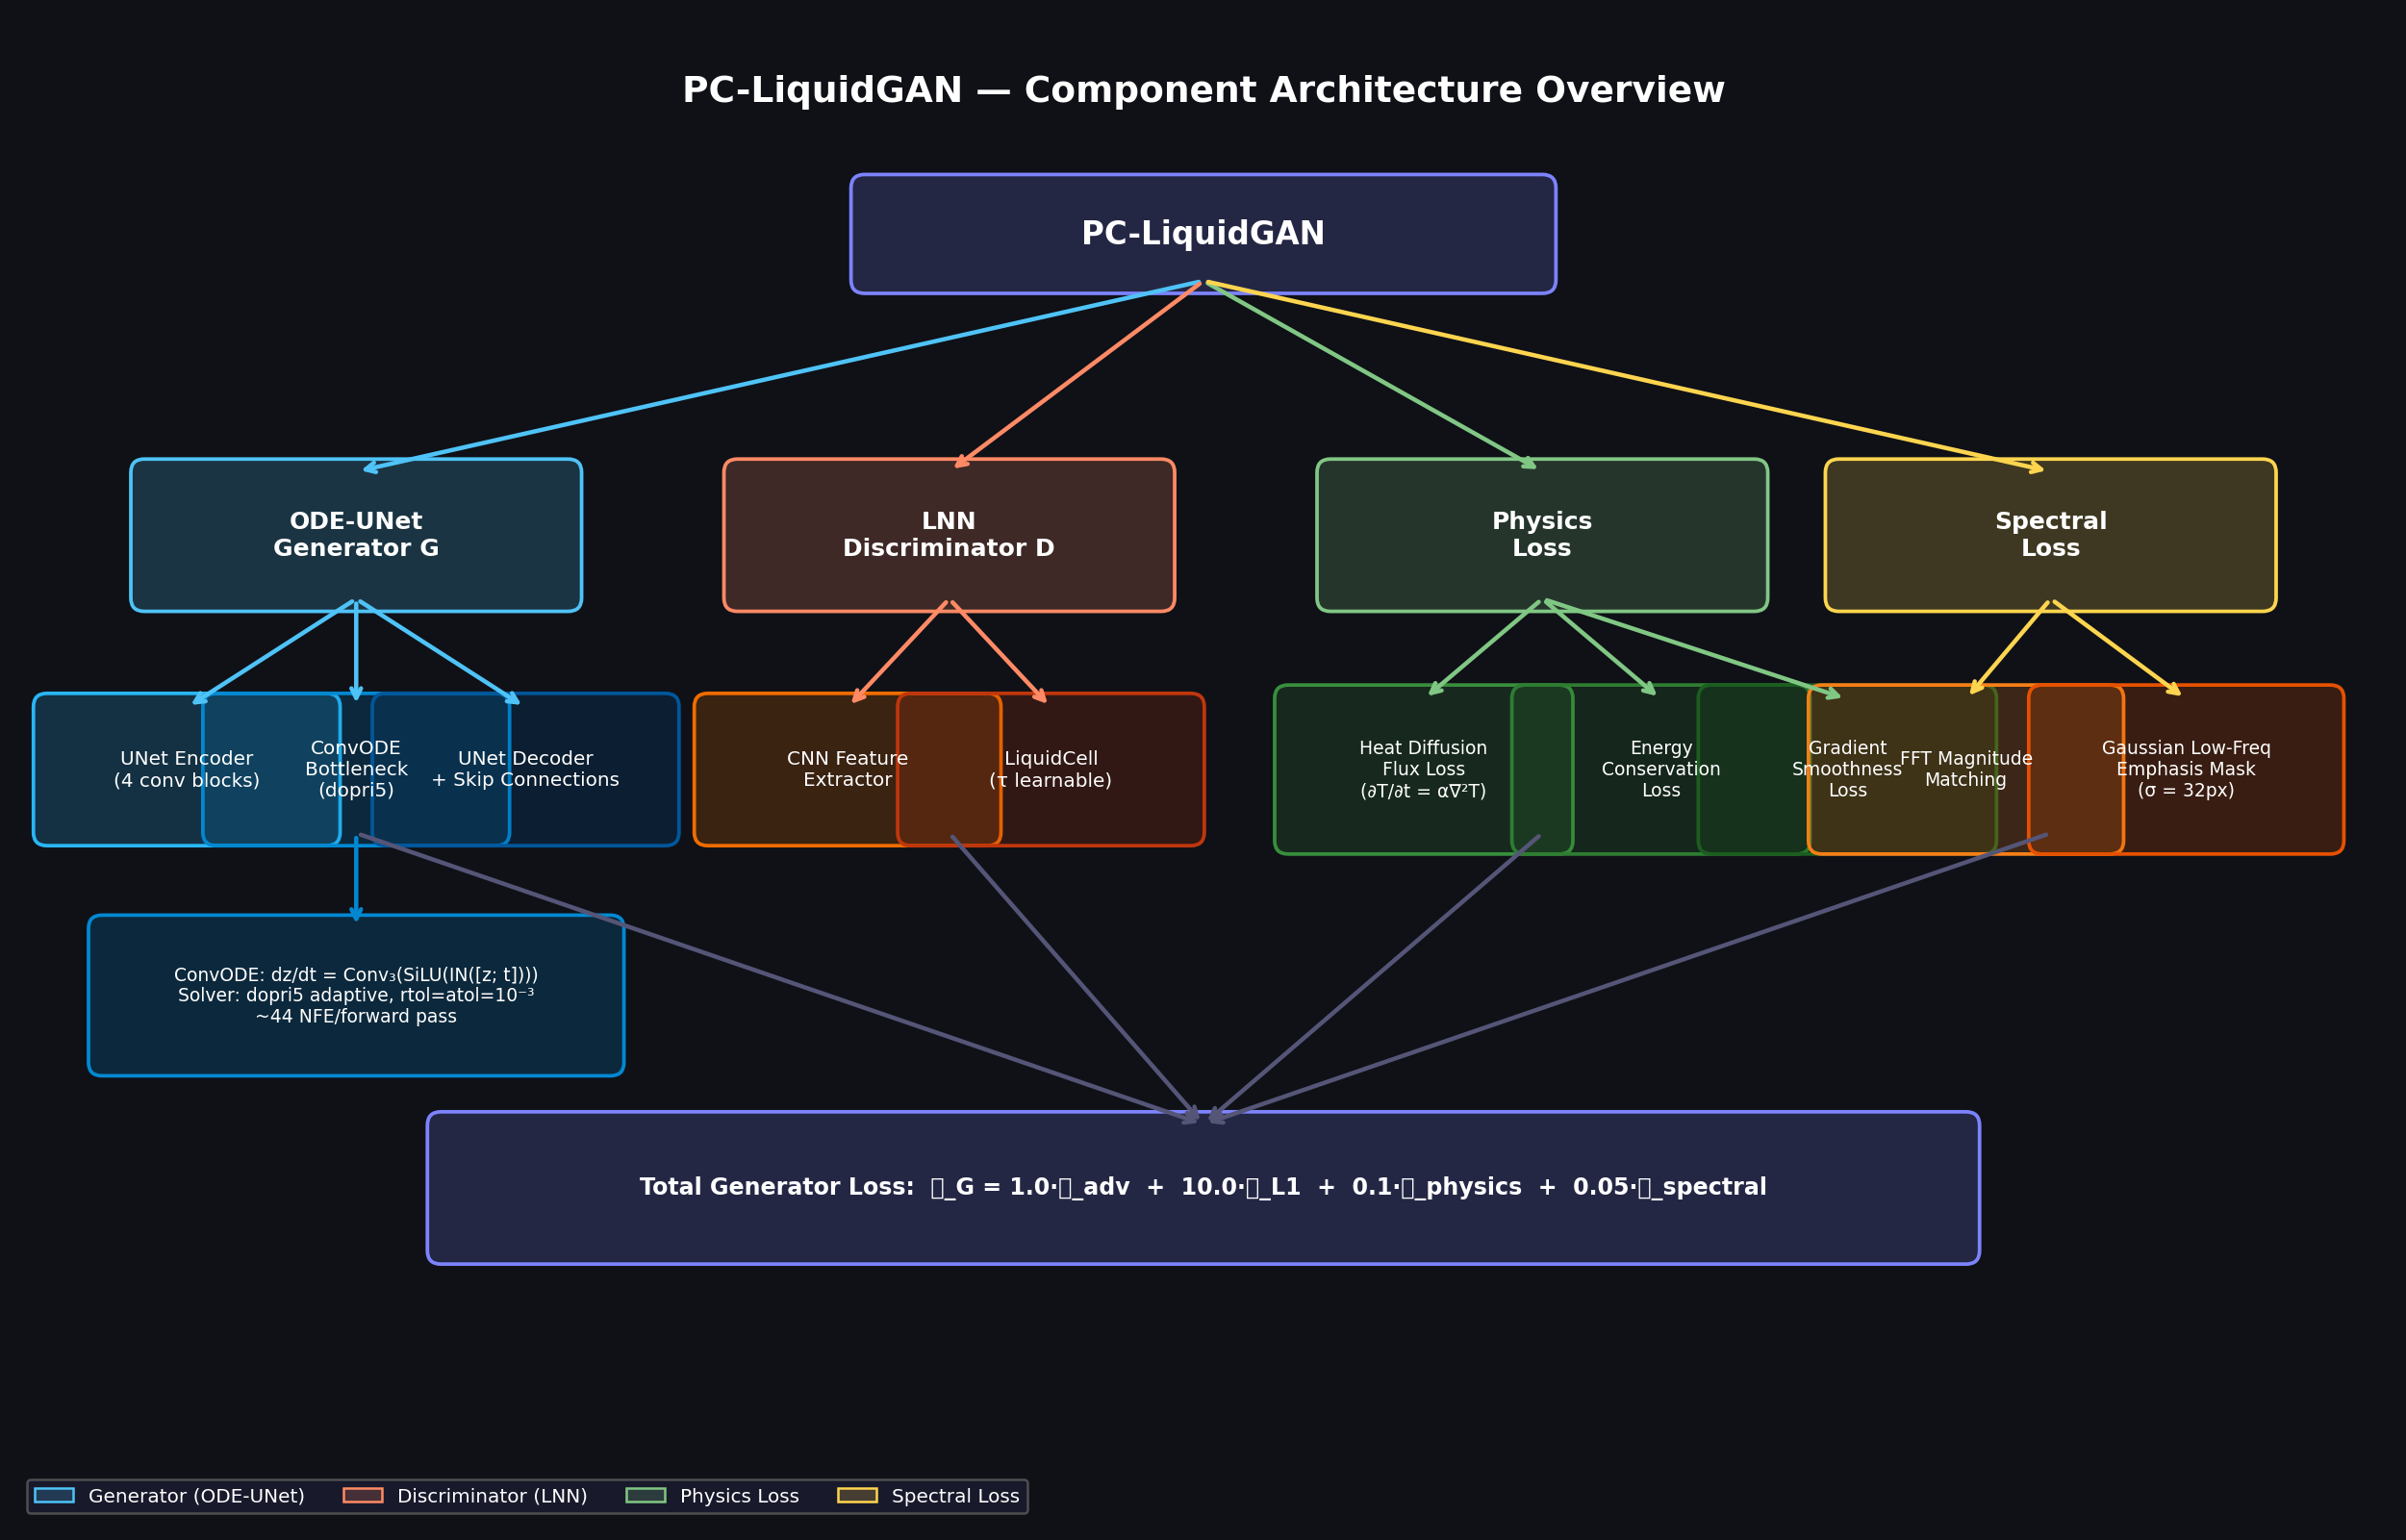
\includegraphics[width=\linewidth]{project_tree.png}
    \caption{Component architecture tree of the proposed PC-LiquidGAN framework, showing the four major subsystems: ODE-UNet Generator, Liquid Neural Network Discriminator, Physics-Constrained Loss, and FFT Spectral Loss.}
    \label{fig:project_tree}
\end{figure}

\section{Neural Ordinary Differential Equations}

Chen et al.~\cite{b_neuralode} introduced Neural ODEs as a continuous-depth generalisation of ResNets. Instead of computing discrete layer transformations $\mathbf{h}_{t+1} = \mathbf{h}_t + f(\mathbf{h}_t)$, a Neural ODE parameterises the \emph{derivative} of the hidden state:
\begin{equation}
    \frac{d\mathbf{z}}{dt} = f_\theta(t, \mathbf{z}), \quad \mathbf{z}(1) = \mathbf{z}(0) + \int_0^1 f_\theta(t, \mathbf{z})\, dt
\end{equation}
The integral is solved by an ODE solver. Memory-efficient backpropagation is performed via the adjoint sensitivity method, avoiding storing intermediate activations for all solver steps. The adaptive Dormand-Prince solver (dopri5) automatically adjusts step sizes to control local truncation error, concentrating computation in regions of high curvature.

In the context of thermal image synthesis, the Neural ODE provides a natural inductive bias: the latent state evolves continuously, mirroring the continuous diffusion of heat through a physical medium.

\section{Liquid Neural Networks}

Hasani et al.~\cite{b_lnn} introduced Liquid Time-Constant Networks (LTCs), inspired by the neural circuits of C.\ elegans. The key innovation is a learnable per-neuron time constant $\tau$, making the hidden state dynamics:
\begin{equation}
    \tau \frac{d\mathbf{h}}{dt} = -\mathbf{h} + \sigma(\mathbf{W}_{in}\mathbf{x} + \mathbf{W}_{rec}\mathbf{h} + \mathbf{b})
\end{equation}
Rather than a fixed integration speed, each neuron learns how quickly it should respond to inputs. This provides greater expressiveness than standard RNNs with the same parameter count, and demonstrated robustness to distributional shifts in robotic control tasks~\cite{b_lnn2}. In our discriminator, the learnable $\tau$ enables adaptive sensitivity to different temporal scales of thermal texture.

\section{Physics-Informed Neural Networks}

Raissi et al.~\cite{b_pinn} proposed Physics-Informed Neural Networks (PINNs), embedding governing PDEs as residual loss terms during training. For a PDE $\mathcal{N}[u] = f$ (where $\mathcal{N}$ is a differential operator), the network is penalised proportionally to the residual $\|\ \mathcal{N}[u_\theta] - f\|^2$, minimised simultaneously with data-fitting. This approach has been highly successful in scientific computing for solving forward and inverse PDE problems with limited data. Our work is the first to apply PDE residual losses within an adversarial generative framework for thermal image synthesis.

\section{Frequency-Domain Learning}

Frequency-domain supervision has been explored in image restoration~\cite{b_fft1} and super-resolution tasks. The physical basis for applying frequency constraints to thermal images is well-established: solutions to the heat diffusion PDE are inherently low-frequency dominant, as the diffusion operator acts as a spatial low-pass filter. Matching the FFT magnitude spectrum of generated and real images provides a direct, frequency-aware constraint that pixel-space L1/L2 losses cannot enforce.

\section{Research Gaps}

Based on the reviewed literature, five key research gaps motivate this work:

\begin{itemize}
    \item \textbf{G1.} No prior work combines Neural ODEs with UNet skip connections for thermal image synthesis, addressing the catastrophic spatial information loss in flat-latent ODE generators.
    \item \textbf{G2.} No prior thermal synthesis GAN incorporates a heat diffusion PDE residual loss.
    \item \textbf{G3.} LNN-based discriminators have not been evaluated alongside physics-informed generative objectives.
    \item \textbf{G4.} The benefit of adaptive ODE solvers (dopri5) over fixed-step solvers (RK4) in GAN training has not been quantified.
    \item \textbf{G5.} Cross-domain zero-shot thermal generalisation of physics-informed models has not been studied.
\end{itemize}